% Generated by pysimcount.figleader -- do not edit; regenerate instead.
% figure: main-t-all-formulas -- source curves (no error bars) with n = 180..525 enlarged
% seeds [1, 2, 3, 4, 5, 6, 7, 8, 9, 10]; metric=t kind=xyz merged (Clifford+T (ct), simcount template)
% shown: suzuki4, suzuki6, mo-q6, mo-q14, bm-q10, mo-o8-q21, morales-y8m10, morales-m8
% removed (see main-t-all-formulas-ranking.md): lie-trotter, suzuki2, suzuki8
% left axis: coordinates copied unchanged from the source .tex, error bars removed
% right axis: the same coordinates and error bars, clipped to the window
% derived: main-t-all-formulas.tex by pysimcount.figleader; source_sha256=d8bd6c0dba2d0407bbc505b2ea718a06a0b2c6d4823a6af5669c10cbab3c780c
% figure made at git_commit=eed0c490bd2a7ed3c821acf76ae930c79d2195f6 git_dirty=False
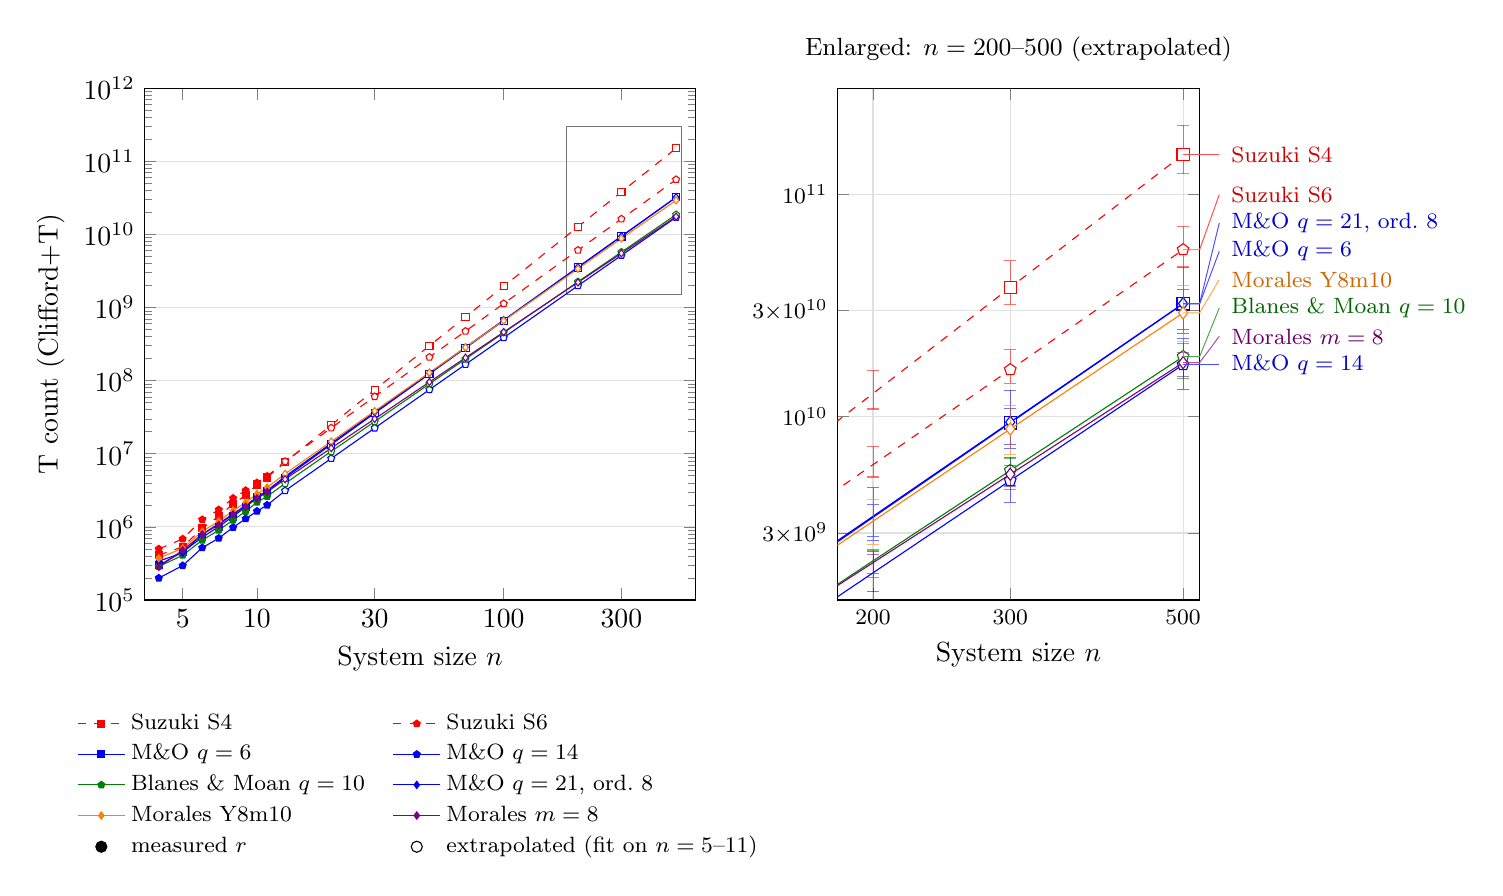
\begin{tikzpicture}
  \begin{loglogaxis}[
    name=main, scale only axis,
    width=7.0cm, height=6.5cm,
    xlabel={System size $n$},
    ylabel={T count (Clifford+T)},
    xtick={5,10,30,100,300}, xticklabels={5,10,30,100,300},
    xmin=3.5, xmax=600, ymin=100000, ymax=1e+12,
    ymajorgrids=true, grid style={black!12},
    legend style={at={(0.5,-0.2)}, anchor=north, draw=none, font=\footnotesize,
      legend columns=2, /tikz/every even column/.append style={column sep=8pt}},
    legend cell align=left,
  ]
    \draw[black!55, line width=0.5pt] (axis cs:180,1.5e+09) rectangle (axis cs:525,3e+11);
    % suzuki4: measured n, mean over seeds, bars min..max over seeds
    \addplot[red, dashed, mark=square*, mark size=1.3pt, mark options={solid, fill=red}] coordinates {
      (4,410227)
      (5,535141)
      (6,956087)
      (7,1.39859e+06)
      (8,2.05215e+06)
      (9,2.71254e+06)
      (10,3.81418e+06)
      (11,4.74467e+06)
    };
    \addlegendentry{Suzuki S4}
    % suzuki4: extrapolated, per-seed fitted r, every step synthesised; mean over seeds, bars min..max
    \addplot[red, dashed, mark=square*, mark size=1.3pt, mark options={solid, fill=white}, mark indices={2,...,10}, forget plot] coordinates {
      (11,4.74467e+06)
      (13,7.66257e+06)
      (20,2.47721e+07)
      (30,7.47488e+07)
      (50,2.99557e+08)
      (70,7.41804e+08)
      (100,1.95329e+09)
      (200,1.27159e+10)
      (300,3.81078e+10)
      (500,1.5088e+11)
    };
    % suzuki6: measured n, mean over seeds, bars min..max over seeds
    \addplot[red, dashed, mark=pentagon*, mark size=1.3pt, mark options={solid, fill=red}] coordinates {
      (4,498655)
      (5,683636)
      (6,1.25709e+06)
      (7,1.71681e+06)
      (8,2.46342e+06)
      (9,3.14791e+06)
      (10,4.01292e+06)
      (11,4.938e+06)
    };
    \addlegendentry{Suzuki S6}
    % suzuki6: extrapolated, per-seed fitted r, every step synthesised; mean over seeds, bars min..max
    \addplot[red, dashed, mark=pentagon*, mark size=1.3pt, mark options={solid, fill=white}, mark indices={2,...,10}, forget plot] coordinates {
      (11,4.938e+06)
      (13,7.85273e+06)
      (20,2.25571e+07)
      (30,6.05362e+07)
      (50,2.09429e+08)
      (70,4.74592e+08)
      (100,1.13273e+09)
      (200,6.08751e+09)
      (300,1.62764e+10)
      (500,5.631e+10)
    };
    % mo-q6: measured n, mean over seeds, bars min..max over seeds
    \addplot[blue, solid, mark=square*, mark size=1.3pt, mark options={solid, fill=blue}] coordinates {
      (4,298204)
      (5,454337)
      (6,719342)
      (7,1.00507e+06)
      (8,1.38971e+06)
      (9,1.87541e+06)
      (10,2.57989e+06)
      (11,3.07213e+06)
    };
    \addlegendentry{M\&O $q=6$}
    % mo-q6: extrapolated, per-seed fitted r, every step synthesised; mean over seeds, bars min..max
    \addplot[blue, solid, mark=square*, mark size=1.3pt, mark options={solid, fill=white}, mark indices={2,...,10}, forget plot] coordinates {
      (11,3.07213e+06)
      (13,4.68293e+06)
      (20,1.33975e+07)
      (30,3.58209e+07)
      (50,1.23593e+08)
      (70,2.79089e+08)
      (100,6.61509e+08)
      (200,3.52821e+09)
      (300,9.37974e+09)
      (500,3.21589e+10)
    };
    % mo-q14: measured n, mean over seeds, bars min..max over seeds
    \addplot[blue, solid, mark=pentagon*, mark size=1.3pt, mark options={solid, fill=blue}] coordinates {
      (4,199644)
      (5,295456)
      (6,517803)
      (7,700110)
      (8,982626)
      (9,1.29212e+06)
      (10,1.63772e+06)
      (11,1.98699e+06)
    };
    \addlegendentry{M\&O $q=14$}
    % mo-q14: extrapolated, per-seed fitted r, every step synthesised; mean over seeds, bars min..max
    \addplot[blue, solid, mark=pentagon*, mark size=1.3pt, mark options={solid, fill=white}, mark indices={2,...,10}, forget plot] coordinates {
      (11,1.98699e+06)
      (13,3.11874e+06)
      (20,8.61978e+06)
      (30,2.2459e+07)
      (50,7.52655e+07)
      (70,1.66795e+08)
      (100,3.86553e+08)
      (200,1.98691e+09)
      (300,5.16555e+09)
      (500,1.71426e+10)
    };
    % bm-q10: measured n, mean over seeds, bars min..max over seeds
    \addplot[green!50!black, solid, mark=pentagon*, mark size=1.3pt, mark options={solid, fill=green!50!black}] coordinates {
      (4,287233)
      (5,408923)
      (6,658784)
      (7,901238)
      (8,1.23945e+06)
      (9,1.62436e+06)
      (10,2.1788e+06)
      (11,2.60871e+06)
    };
    \addlegendentry{Blanes \& Moan $q=10$}
    % bm-q10: extrapolated, per-seed fitted r, every step synthesised; mean over seeds, bars min..max
    \addplot[green!50!black, solid, mark=pentagon*, mark size=1.3pt, mark options={solid, fill=white}, mark indices={2,...,10}, forget plot] coordinates {
      (11,2.60871e+06)
      (13,3.9301e+06)
      (20,1.0774e+07)
      (30,2.7548e+07)
      (50,9.03062e+07)
      (70,1.9751e+08)
      (100,4.51462e+08)
      (200,2.24975e+09)
      (300,5.73099e+09)
      (500,1.86331e+10)
    };
    % mo-o8-q21: measured n, mean over seeds, bars min..max over seeds
    \addplot[blue, solid, mark=diamond*, mark size=1.3pt, mark options={solid, fill=blue}] coordinates {
      (4,338991)
      (5,443831)
      (6,791120)
      (7,1.1119e+06)
      (8,1.50621e+06)
      (9,1.97285e+06)
      (10,2.54893e+06)
      (11,3.13956e+06)
    };
    \addlegendentry{M\&O $q=21$, ord.~8}
    % mo-o8-q21: extrapolated, per-seed fitted r, every step synthesised; mean over seeds, bars min..max
    \addplot[blue, solid, mark=diamond*, mark size=1.3pt, mark options={solid, fill=white}, mark indices={2,...,10}, forget plot] coordinates {
      (11,3.13956e+06)
      (13,4.88976e+06)
      (20,1.39079e+07)
      (30,3.70353e+07)
      (50,1.2702e+08)
      (70,2.85327e+08)
      (100,6.73578e+08)
      (200,3.56917e+09)
      (300,9.45042e+09)
      (500,3.22461e+10)
    };
    % morales-y8m10: measured n, mean over seeds, bars min..max over seeds
    \addplot[orange, solid, mark=diamond*, mark size=1.3pt, mark options={solid, fill=orange}] coordinates {
      (4,373838)
      (5,509327)
      (6,864458)
      (7,1.19952e+06)
      (8,1.66587e+06)
      (9,2.15577e+06)
      (10,2.81799e+06)
      (11,3.46189e+06)
    };
    \addlegendentry{Morales Y8m10}
    % morales-y8m10: extrapolated, per-seed fitted r, every step synthesised; mean over seeds, bars min..max
    \addplot[orange, solid, mark=diamond*, mark size=1.3pt, mark options={solid, fill=white}, mark indices={2,...,10}, forget plot] coordinates {
      (11,3.46189e+06)
      (13,5.32463e+06)
      (20,1.47085e+07)
      (30,3.84186e+07)
      (50,1.28596e+08)
      (70,2.84865e+08)
      (100,6.59306e+08)
      (200,3.39046e+09)
      (300,8.80299e+09)
      (500,2.92891e+10)
    };
    % morales-m8: measured n, mean over seeds, bars min..max over seeds
    \addplot[violet, solid, mark=diamond*, mark size=1.3pt, mark options={solid, fill=violet}] coordinates {
      (4,283483)
      (5,480273)
      (6,790926)
      (7,1.06227e+06)
      (8,1.48074e+06)
      (9,1.89288e+06)
      (10,2.4461e+06)
      (11,3.00394e+06)
    };
    \addlegendentry{Morales $m=8$}
    % morales-m8: extrapolated, per-seed fitted r, every step synthesised; mean over seeds, bars min..max
    \addplot[violet, solid, mark=diamond*, mark size=1.3pt, mark options={solid, fill=white}, mark indices={2,...,10}, forget plot] coordinates {
      (11,3.00394e+06)
      (13,4.48114e+06)
      (20,1.19454e+07)
      (30,3.00095e+07)
      (50,9.5688e+07)
      (70,2.05711e+08)
      (100,4.61972e+08)
      (200,2.2065e+09)
      (300,5.51227e+09)
      (500,1.75035e+10)
    };
    \addlegendimage{only marks, black, mark=*, mark options={solid, fill=black}}
    \addlegendentry{measured $r$}
    \addlegendimage{only marks, black, mark=*, mark options={solid, fill=white}}
    \addlegendentry{extrapolated (fit on $n = 5$--$11$)}
  \end{loglogaxis}
  \begin{loglogaxis}[
    scale only axis,
    at={(8.8cm,0cm)}, anchor=south west,
    width=4.6cm, height=6.5cm,
    title={Enlarged: $n = 200$--$500$ (extrapolated)}, title style={font=\small},
    xlabel={System size $n$},
    xtick={200,300,500}, xticklabels={200,300,500}, xminorticks=false,
    ytick={3e+09,1e+10,3e+10,1e+11}, yticklabels={{$3{\times}10^{9}$},{$10^{10}$},{$3{\times}10^{10}$},{$10^{11}$}}, yminorticks=false,
    xmin=180, xmax=525, ymin=1.5e+09, ymax=3e+11,
    xmajorgrids=true, ymajorgrids=true, grid style={black!12}, tick label style={font=\footnotesize},
    clip mode=individual,
  ]
    % suzuki4: extrapolated, per-seed fitted r, every step synthesised; mean over seeds, bars min..max
    \addplot[red, dashed, mark=square*, mark size=2.2pt, mark options={solid, fill=white}, mark indices={2,...,10}, forget plot, error bars/.cd, y dir=both, y explicit, error bar style={solid, line width=0.35pt, opacity=0.55}] coordinates {
      (11,4.74467e+06)
      (13,7.66257e+06) += (0,387782) -= (0,206484)
      (20,2.47721e+07) += (0,2.00435e+06) -= (0,1.20859e+06)
      (30,7.47488e+07) += (0,8.81613e+06) -= (0,6.58761e+06)
      (50,2.99557e+08) += (0,4.65816e+07) -= (0,2.86018e+07)
      (70,7.41804e+08) += (0,1.31839e+08) -= (0,7.07925e+07)
      (100,1.95329e+09) += (0,4.06516e+08) -= (0,2.27538e+08)
      (200,1.27159e+10) += (0,3.44947e+09) -= (0,1.88592e+09)
      (300,3.81078e+10) += (0,1.21917e+10) -= (0,6.09671e+09)
      (500,1.5088e+11) += (0,5.3077e+10) -= (0,2.70956e+10)
    };
    % suzuki6: extrapolated, per-seed fitted r, every step synthesised; mean over seeds, bars min..max
    \addplot[red, dashed, mark=pentagon*, mark size=2.2pt, mark options={solid, fill=white}, mark indices={2,...,10}, forget plot, error bars/.cd, y dir=both, y explicit, error bar style={solid, line width=0.35pt, opacity=0.55}] coordinates {
      (11,4.938e+06)
      (13,7.85273e+06) += (0,300450) -= (0,160976)
      (20,2.25571e+07) += (0,1.11956e+06) -= (0,1.00763e+06)
      (30,6.05362e+07) += (0,3.59495e+06) -= (0,2.84472e+06)
      (50,2.09429e+08) += (0,1.94953e+07) -= (0,1.38993e+07)
      (70,4.74592e+08) += (0,6.38993e+07) -= (0,3.83182e+07)
      (100,1.13273e+09) += (0,1.64668e+08) -= (0,1.01944e+08)
      (200,6.08751e+09) += (0,1.27029e+09) -= (0,7.27509e+08)
      (300,1.62764e+10) += (0,3.70913e+09) -= (0,2.14677e+09)
      (500,5.631e+10) += (0,1.54407e+10) -= (0,8.83844e+09)
    };
    % mo-q6: extrapolated, per-seed fitted r, every step synthesised; mean over seeds, bars min..max
    \addplot[blue, solid, mark=square*, mark size=2.2pt, mark options={solid, fill=white}, mark indices={2,...,10}, forget plot, error bars/.cd, y dir=both, y explicit, error bar style={solid, line width=0.35pt, opacity=0.55}] coordinates {
      (11,3.07213e+06)
      (13,4.68293e+06) += (0,356548) -= (0,198754)
      (20,1.33975e+07) += (0,1.57555e+06) -= (0,835830)
      (30,3.58209e+07) += (0,5.86251e+06) -= (0,3.55025e+06)
      (50,1.23593e+08) += (0,2.50475e+07) -= (0,1.49872e+07)
      (70,2.79089e+08) += (0,7.04831e+07) -= (0,4.14157e+07)
      (100,6.61509e+08) += (0,1.94197e+08) -= (0,1.14688e+08)
      (200,3.52821e+09) += (0,1.26118e+09) -= (0,7.4489e+08)
      (300,9.37974e+09) += (0,3.79409e+09) -= (0,2.16652e+09)
      (500,3.21589e+10) += (0,1.48961e+10) -= (0,8.4356e+09)
    };
    % mo-q14: extrapolated, per-seed fitted r, every step synthesised; mean over seeds, bars min..max
    \addplot[blue, solid, mark=pentagon*, mark size=2.2pt, mark options={solid, fill=white}, mark indices={2,...,10}, forget plot, error bars/.cd, y dir=both, y explicit, error bar style={solid, line width=0.35pt, opacity=0.55}] coordinates {
      (11,1.98699e+06)
      (13,3.11874e+06) += (0,57718.4) -= (0,105462)
      (20,8.61978e+06) += (0,566221) -= (0,428091)
      (30,2.2459e+07) += (0,2.19943e+06) -= (0,1.58811e+06)
      (50,7.52655e+07) += (0,9.82788e+06) -= (0,7.79298e+06)
      (70,1.66795e+08) += (0,2.71474e+07) -= (0,2.02453e+07)
      (100,3.86553e+08) += (0,7.14752e+07) -= (0,5.46946e+07)
      (200,1.98691e+09) += (0,4.88484e+08) -= (0,3.55086e+08)
      (300,5.16555e+09) += (0,1.40651e+09) -= (0,1.03303e+09)
      (500,1.71426e+10) += (0,5.38038e+09) -= (0,3.83706e+09)
    };
    % bm-q10: extrapolated, per-seed fitted r, every step synthesised; mean over seeds, bars min..max
    \addplot[green!50!black, solid, mark=pentagon*, mark size=2.2pt, mark options={solid, fill=white}, mark indices={2,...,10}, forget plot, error bars/.cd, y dir=both, y explicit, error bar style={solid, line width=0.35pt, opacity=0.55}] coordinates {
      (11,2.60871e+06)
      (13,3.9301e+06) += (0,68836) -= (0,87804)
      (20,1.0774e+07) += (0,460669) -= (0,649855)
      (30,2.7548e+07) += (0,1.70443e+06) -= (0,1.9026e+06)
      (50,9.03062e+07) += (0,6.58258e+06) -= (0,8.73882e+06)
      (70,1.9751e+08) += (0,1.7158e+07) -= (0,2.14673e+07)
      (100,4.51462e+08) += (0,4.29653e+07) -= (0,5.62649e+07)
      (200,2.24975e+09) += (0,2.68432e+08) -= (0,3.56254e+08)
      (300,5.73099e+09) += (0,7.68518e+08) -= (0,1.04131e+09)
      (500,1.86331e+10) += (0,2.68049e+09) -= (0,3.81581e+09)
    };
    % mo-o8-q21: extrapolated, per-seed fitted r, every step synthesised; mean over seeds, bars min..max
    \addplot[blue, solid, mark=diamond*, mark size=2.2pt, mark options={solid, fill=white}, mark indices={2,...,10}, forget plot, error bars/.cd, y dir=both, y explicit, error bar style={solid, line width=0.35pt, opacity=0.55}] coordinates {
      (11,3.13956e+06)
      (13,4.88976e+06) += (0,56791) -= (0,186319)
      (20,1.39079e+07) += (0,486906) -= (0,907256)
      (30,3.70353e+07) += (0,1.60026e+06) -= (0,3.14339e+06)
      (50,1.2702e+08) += (0,8.2286e+06) -= (0,1.46677e+07)
      (70,2.85327e+08) += (0,2.31775e+07) -= (0,3.56762e+07)
      (100,6.73578e+08) += (0,6.27389e+07) -= (0,1.02361e+08)
      (200,3.56917e+09) += (0,4.59913e+08) -= (0,6.71365e+08)
      (300,9.45042e+09) += (0,1.40818e+09) -= (0,1.97079e+09)
      (500,3.22461e+10) += (0,5.17455e+09) -= (0,7.59363e+09)
    };
    % morales-y8m10: extrapolated, per-seed fitted r, every step synthesised; mean over seeds, bars min..max
    \addplot[orange, solid, mark=diamond*, mark size=2.2pt, mark options={solid, fill=white}, mark indices={2,...,10}, forget plot, error bars/.cd, y dir=both, y explicit, error bar style={solid, line width=0.35pt, opacity=0.55}] coordinates {
      (11,3.46189e+06)
      (13,5.32463e+06) += (0,272075) -= (0,227581)
      (20,1.47085e+07) += (0,1.14689e+06) -= (0,1.13279e+06)
      (30,3.84186e+07) += (0,3.78324e+06) -= (0,3.5671e+06)
      (50,1.28596e+08) += (0,1.83792e+07) -= (0,1.61923e+07)
      (70,2.84865e+08) += (0,4.67169e+07) -= (0,4.26348e+07)
      (100,6.59306e+08) += (0,1.2942e+08) -= (0,1.13282e+08)
      (200,3.39046e+09) += (0,8.63829e+08) -= (0,7.1373e+08)
      (300,8.80299e+09) += (0,2.42332e+09) -= (0,2.02459e+09)
      (500,2.92891e+10) += (0,9.53382e+09) -= (0,7.5792e+09)
    };
    % morales-m8: extrapolated, per-seed fitted r, every step synthesised; mean over seeds, bars min..max
    \addplot[violet, solid, mark=diamond*, mark size=2.2pt, mark options={solid, fill=white}, mark indices={2,...,10}, forget plot, error bars/.cd, y dir=both, y explicit, error bar style={solid, line width=0.35pt, opacity=0.55}] coordinates {
      (11,3.00394e+06)
      (13,4.48114e+06) += (0,71643.2) -= (0,105161)
      (20,1.19454e+07) += (0,365553) -= (0,348003)
      (30,3.00095e+07) += (0,1.1417e+06) -= (0,1.11385e+06)
      (50,9.5688e+07) += (0,5.37813e+06) -= (0,4.85e+06)
      (70,2.05711e+08) += (0,1.29501e+07) -= (0,1.22873e+07)
      (100,4.61972e+08) += (0,3.26388e+07) -= (0,3.73721e+07)
      (200,2.2065e+09) += (0,1.93245e+08) -= (0,2.24446e+08)
      (300,5.51227e+09) += (0,5.39536e+08) -= (0,6.30311e+08)
      (500,1.75035e+10) += (0,1.90596e+09) -= (0,2.33772e+09)
    };
    \draw[red!70, line width=0.35pt] (axis cs:500,1.5088e+11) -- (axis cs:525,1.5088e+11) -- ([xshift=0.25cm]axis cs:525,1.5088e+11);
    \node[anchor=west, font=\footnotesize, text=red!80!black] at ([xshift=0.28cm]axis cs:525,1.5088e+11) {Suzuki S4};
    \draw[red!70, line width=0.35pt] (axis cs:500,5.631e+10) -- (axis cs:525,5.631e+10) -- ([xshift=0.25cm]axis cs:525,9.97072e+10);
    \node[anchor=west, font=\footnotesize, text=red!80!black] at ([xshift=0.28cm]axis cs:525,9.97072e+10) {Suzuki S6};
    \draw[blue!70, line width=0.35pt] (axis cs:500,3.21589e+10) -- (axis cs:525,3.21589e+10) -- ([xshift=0.25cm]axis cs:525,5.54426e+10);
    \node[anchor=west, font=\footnotesize, text=blue!80!black] at ([xshift=0.28cm]axis cs:525,5.54426e+10) {M\&O $q=6$};
    \draw[blue!70, line width=0.35pt] (axis cs:500,1.71426e+10) -- (axis cs:525,1.71426e+10) -- ([xshift=0.25cm]axis cs:525,1.71426e+10);
    \node[anchor=west, font=\footnotesize, text=blue!80!black] at ([xshift=0.28cm]axis cs:525,1.71426e+10) {M\&O $q=14$};
    \draw[green!50!black!70, line width=0.35pt] (axis cs:500,1.86331e+10) -- (axis cs:525,1.86331e+10) -- ([xshift=0.25cm]axis cs:525,3.0829e+10);
    \node[anchor=west, font=\footnotesize, text=green!50!black!80!black] at ([xshift=0.28cm]axis cs:525,3.0829e+10) {Blanes \& Moan $q=10$};
    \draw[blue!70, line width=0.35pt] (axis cs:500,3.22461e+10) -- (axis cs:525,3.22461e+10) -- ([xshift=0.25cm]axis cs:525,7.43507e+10);
    \node[anchor=west, font=\footnotesize, text=blue!80!black] at ([xshift=0.28cm]axis cs:525,7.43507e+10) {M\&O $q=21$, ord.~8};
    \draw[orange!70, line width=0.35pt] (axis cs:500,2.92891e+10) -- (axis cs:525,2.92891e+10) -- ([xshift=0.25cm]axis cs:525,4.1343e+10);
    \node[anchor=west, font=\footnotesize, text=orange!80!black] at ([xshift=0.28cm]axis cs:525,4.1343e+10) {Morales Y8m10};
    \draw[violet!70, line width=0.35pt] (axis cs:500,1.75035e+10) -- (axis cs:525,1.75035e+10) -- ([xshift=0.25cm]axis cs:525,2.29889e+10);
    \node[anchor=west, font=\footnotesize, text=violet!80!black] at ([xshift=0.28cm]axis cs:525,2.29889e+10) {Morales $m=8$};
  \end{loglogaxis}
\end{tikzpicture}
